% Important: If latex complains about unicode characters,
% please use "\usepackage[utf8x]{inputenc}" in your preamble
% You can change the size of the picture by putting it into the construct:
% 1) \resizebox{10cm}{!}{"below picture"} to scale horizontally to 10 cm
% 2) \resizebox{!}{15cm}{"below picture"} to scale vertically to 15 cm
% 3) \resizebox{10cm}{15cm}{"below picture"} a combination of above two
% It is not recomended to use the scale option of the tikzpicture environment.
\resizebox{15cm}{!}{
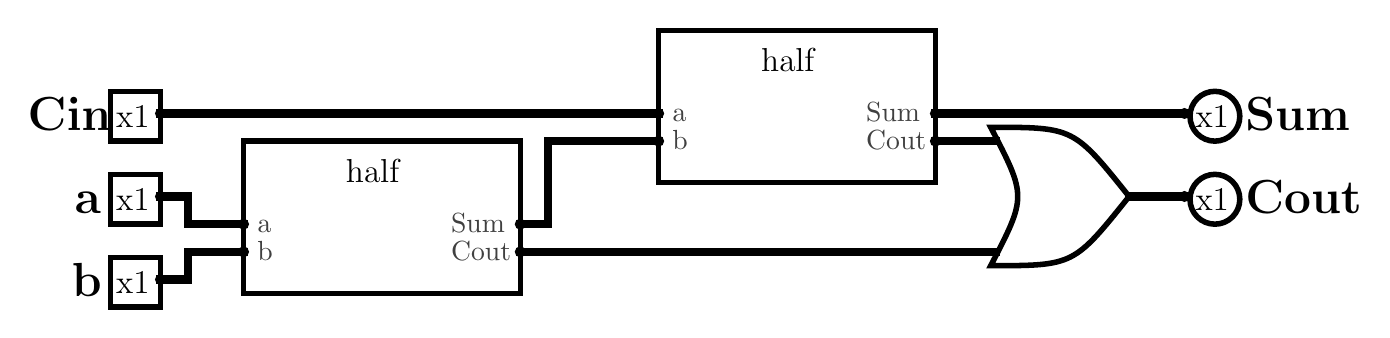
\begin{tikzpicture}[x=1pt,y=-1pt,line cap=rect]
\def\logisimfontA#1{\fontfamily{cmr}{#1}} % Replaced by logisim, original font was "SansSerif"
\definecolor{custcol_0_0_0}{RGB}{0, 0, 0}
\definecolor{custcol_40_40_40}{RGB}{64, 64, 64}
\definecolor{custcol_ff_ff_ff}{RGB}{255, 255, 255}
\draw [line width=3.0pt, custcol_0_0_0 ]  (333.0,36.0) -- (423.0,36.0) ;
\draw [line width=3.0pt, custcol_0_0_0 ]  (403.0,66.0) -- (423.0,66.0) ;
\draw [line width=3.0pt, custcol_0_0_0 ]  (53.0,36.0) -- (233.0,36.0) ;
\draw [line width=3.0pt, custcol_0_0_0 ]  (53.0,66.0) -- (63.0,66.0) -- (63.0,76.0) -- (83.0,76.0) ;
\draw [line width=3.0pt, custcol_0_0_0 ]  (53.0,96.0) -- (63.0,96.0) -- (63.0,86.0) -- (83.0,86.0) ;
\draw [line width=3.0pt, custcol_0_0_0 ]  (183.0,76.0) -- (193.0,76.0) -- (193.0,46.0) -- (233.0,46.0) ;
\draw [line width=2.0pt, custcol_0_0_0 ]  (233.0,6.0) -- (332.0,6.0) ;
\draw [line width=2.0pt, custcol_0_0_0 ]  (333.0,6.0) -- (333.0,60.0) ;
\draw [line width=2.0pt, custcol_0_0_0 ]  (333.0,61.0) -- (234.0,61.0) ;
\draw [line width=2.0pt, custcol_0_0_0 ]  (233.0,61.0) -- (233.0,7.0) ;
\logisimfontA{\fontsize{10pt}{10pt}\selectfont\node[inner sep=0, outer sep=0, custcol_40_40_40, anchor=base west] at  (238.0,39.0)  {a};}
\logisimfontA{\fontsize{10pt}{10pt}\selectfont\node[inner sep=0, outer sep=0, custcol_40_40_40, anchor=base west] at  (238.0,49.0)  {b};}
\logisimfontA{\fontsize{10pt}{10pt}\selectfont\node[inner sep=0, outer sep=0, custcol_40_40_40, anchor=base west] at  (308.0,39.0)  {Sum};}
\logisimfontA{\fontsize{10pt}{10pt}\selectfont\node[inner sep=0, outer sep=0, custcol_40_40_40, anchor=base west] at  (308.0,49.0)  {Cout};}
\logisimfontA{\fontsize{12pt}{12pt}\selectfont\node[inner sep=0, outer sep=0, custcol_0_0_0, anchor=base west] at  (270.0,21.0)  {half};}
\fill [line width=1.0pt, custcol_0_0_0]  (233.0,36.0) ellipse (2.0 and 2.0 );
\fill [line width=1.0pt, custcol_0_0_0]  (233.0,46.0) ellipse (2.0 and 2.0 );
\fill [line width=1.0pt, custcol_0_0_0]  (333.0,36.0) ellipse (2.0 and 2.0 );
\fill [line width=1.0pt, custcol_0_0_0]  (333.0,46.0) ellipse (2.0 and 2.0 );
\draw [line width=2.0pt, custcol_0_0_0 ]  (83.0,46.0) -- (182.0,46.0) ;
\draw [line width=2.0pt, custcol_0_0_0 ]  (183.0,46.0) -- (183.0,100.0) ;
\draw [line width=2.0pt, custcol_0_0_0 ]  (183.0,101.0) -- (84.0,101.0) ;
\draw [line width=2.0pt, custcol_0_0_0 ]  (83.0,101.0) -- (83.0,47.0) ;
\logisimfontA{\fontsize{10pt}{10pt}\selectfont\node[inner sep=0, outer sep=0, custcol_40_40_40, anchor=base west] at  (88.0,79.0)  {a};}
\logisimfontA{\fontsize{10pt}{10pt}\selectfont\node[inner sep=0, outer sep=0, custcol_40_40_40, anchor=base west] at  (88.0,89.0)  {b};}
\logisimfontA{\fontsize{10pt}{10pt}\selectfont\node[inner sep=0, outer sep=0, custcol_40_40_40, anchor=base west] at  (158.0,79.0)  {Sum};}
\logisimfontA{\fontsize{10pt}{10pt}\selectfont\node[inner sep=0, outer sep=0, custcol_40_40_40, anchor=base west] at  (158.0,89.0)  {Cout};}
\logisimfontA{\fontsize{12pt}{12pt}\selectfont\node[inner sep=0, outer sep=0, custcol_0_0_0, anchor=base west] at  (120.0,61.0)  {half};}
\fill [line width=1.0pt, custcol_0_0_0]  (83.0,76.0) ellipse (2.0 and 2.0 );
\fill [line width=1.0pt, custcol_0_0_0]  (83.0,86.0) ellipse (2.0 and 2.0 );
\fill [line width=1.0pt, custcol_0_0_0]  (183.0,76.0) ellipse (2.0 and 2.0 );
\fill [line width=1.0pt, custcol_0_0_0]  (183.0,86.0) ellipse (2.0 and 2.0 );
\draw [line width=2.0pt, custcol_0_0_0 ]  (35.0,28.0) -- (52.0,28.0) ;
\draw [line width=2.0pt, custcol_0_0_0 ]  (53.0,28.0) -- (53.0,45.0) ;
\draw [line width=2.0pt, custcol_0_0_0 ]  (53.0,46.0) -- (36.0,46.0) ;
\draw [line width=2.0pt, custcol_0_0_0 ]  (35.0,46.0) -- (35.0,29.0) ;
\logisimfontA{\fontsize{12pt}{12pt}\selectfont\node[inner sep=0, outer sep=0, custcol_0_0_0, anchor=base west] at  (37.0,41.0)  {x1};}
\logisimfontA{\fontsize{16pt}{16pt}\fontseries{bx}\selectfont\node[inner sep=0, outer sep=0, custcol_0_0_0, anchor=base west] at  (5.0,42.0)  {Cin};}
\fill [line width=2.0pt, custcol_0_0_0]  (53.0,36.0) ellipse (2.0 and 2.0 );
\draw [line width=2.0pt, custcol_0_0_0 ]  (35.0,58.0) -- (52.0,58.0) ;
\draw [line width=2.0pt, custcol_0_0_0 ]  (53.0,58.0) -- (53.0,75.0) ;
\draw [line width=2.0pt, custcol_0_0_0 ]  (53.0,76.0) -- (36.0,76.0) ;
\draw [line width=2.0pt, custcol_0_0_0 ]  (35.0,76.0) -- (35.0,59.0) ;
\logisimfontA{\fontsize{12pt}{12pt}\selectfont\node[inner sep=0, outer sep=0, custcol_0_0_0, anchor=base west] at  (37.0,71.0)  {x1};}
\logisimfontA{\fontsize{16pt}{16pt}\fontseries{bx}\selectfont\node[inner sep=0, outer sep=0, custcol_0_0_0, anchor=base west] at  (22.0,72.0)  {a};}
\fill [line width=2.0pt, custcol_0_0_0]  (53.0,66.0) ellipse (2.0 and 2.0 );
\draw [line width=2.0pt, custcol_0_0_0 ]  (35.0,88.0) -- (52.0,88.0) ;
\draw [line width=2.0pt, custcol_0_0_0 ]  (53.0,88.0) -- (53.0,105.0) ;
\draw [line width=2.0pt, custcol_0_0_0 ]  (53.0,106.0) -- (36.0,106.0) ;
\draw [line width=2.0pt, custcol_0_0_0 ]  (35.0,106.0) -- (35.0,89.0) ;
\logisimfontA{\fontsize{12pt}{12pt}\selectfont\node[inner sep=0, outer sep=0, custcol_0_0_0, anchor=base west] at  (37.0,101.0)  {x1};}
\logisimfontA{\fontsize{16pt}{16pt}\fontseries{bx}\selectfont\node[inner sep=0, outer sep=0, custcol_0_0_0, anchor=base west] at  (21.0,102.0)  {b};}
\fill [line width=2.0pt, custcol_0_0_0]  (53.0,96.0) ellipse (2.0 and 2.0 );
\draw [line width=3.0pt, custcol_0_0_0 ]  (333.0,46.0) -- (353.0,46.0) -- (355.0,46.0) ;
\draw [line width=3.0pt, custcol_0_0_0 ]  (183.0,86.0) -- (353.0,86.0) -- (355.0,86.0) ;
\draw [line width=2.0pt, custcol_0_0_0 ]  (403.0,66.0) .. controls  (383.0,41.0)  ..  (353.0,41.0) .. controls  (366.0,66.0)  ..  (353.0,91.0) .. controls  (383.0,91.0)  ..  (403.0,66.0) -- cycle ;
\draw [line width=2.0pt, custcol_0_0_0]  (434.0,67.0) ellipse (9.0 and 9.0 );
\logisimfontA{\fontsize{12pt}{12pt}\selectfont\node[inner sep=0, outer sep=0, custcol_0_0_0, anchor=base west] at  (427.0,71.0)  {x1};}
\logisimfontA{\fontsize{16pt}{16pt}\fontseries{bx}\selectfont\node[inner sep=0, outer sep=0, custcol_0_0_0, anchor=base west] at  (445.0,72.0)  {Cout};}
\fill [line width=2.0pt, custcol_0_0_0]  (423.0,66.0) ellipse (2.0 and 2.0 );
\draw [line width=2.0pt, custcol_0_0_0]  (434.0,37.0) ellipse (9.0 and 9.0 );
\logisimfontA{\fontsize{12pt}{12pt}\selectfont\node[inner sep=0, outer sep=0, custcol_0_0_0, anchor=base west] at  (427.0,41.0)  {x1};}
\logisimfontA{\fontsize{16pt}{16pt}\fontseries{bx}\selectfont\node[inner sep=0, outer sep=0, custcol_0_0_0, anchor=base west] at  (445.0,42.0)  {Sum};}
\fill [line width=2.0pt, custcol_0_0_0]  (423.0,36.0) ellipse (2.0 and 2.0 );
\end{tikzpicture}
}
